\chapter{Теория}
\label{ch:intro}

\begin{figure}[H]
    \centering
    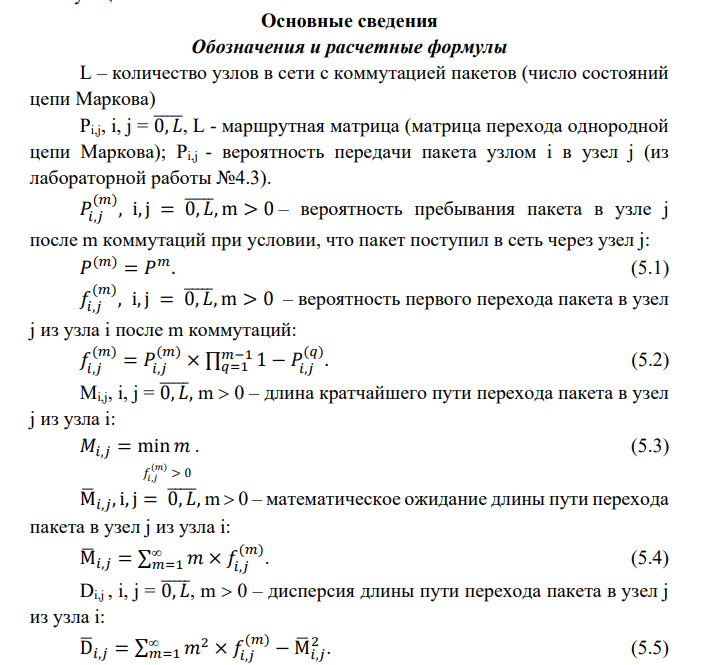
\includegraphics[width=1.0\textwidth]{theory1.png}
    \caption{Теория для лабораторной работы}
\end{figure}

\begin{figure}[H]
    \centering
    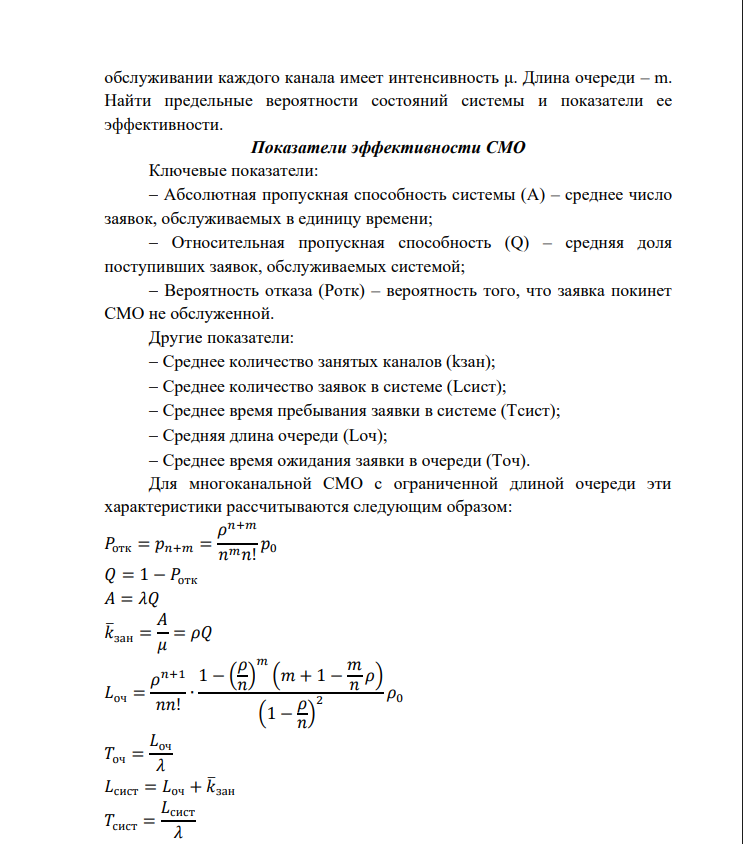
\includegraphics[width=1.0\textwidth]{theory2.png}
    \caption{Теория для лабораторной работы}
\end{figure}

\begin{figure}[H]
    \centering
    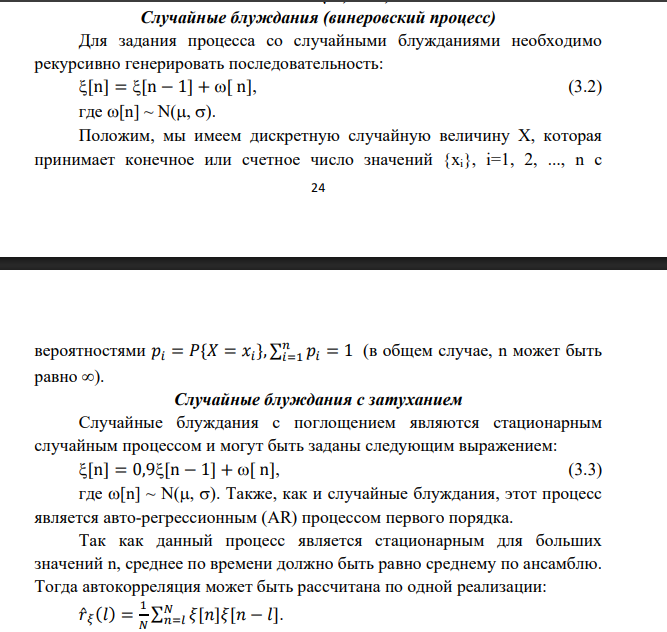
\includegraphics[width=1.0\textwidth]{theory3.png}
    \caption{Теория для лабораторной работы}
\end{figure}

\begin{figure}[H]
    \centering
    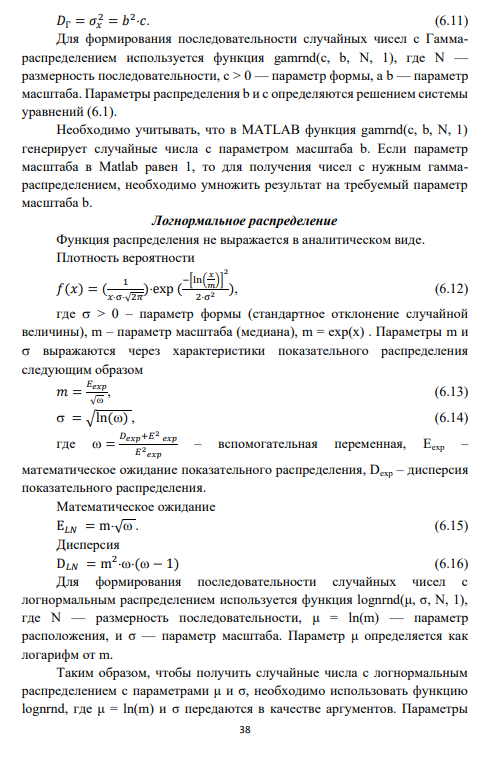
\includegraphics[width=1.0\textwidth]{theory4.png}
    \caption{Теория для лабораторной работы}
\end{figure}

\begin{figure}[H]
    \centering
    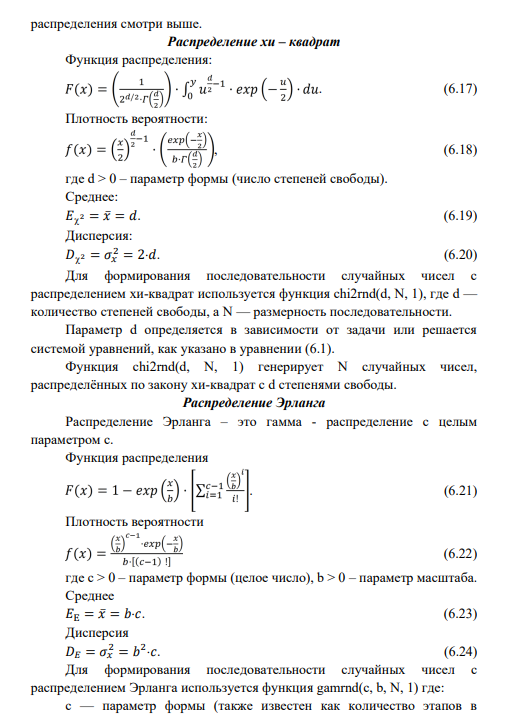
\includegraphics[width=1.0\textwidth]{theory5.png}
    \caption{Теория для лабораторной работы}
\end{figure}

\begin{figure}[H]
    \centering
    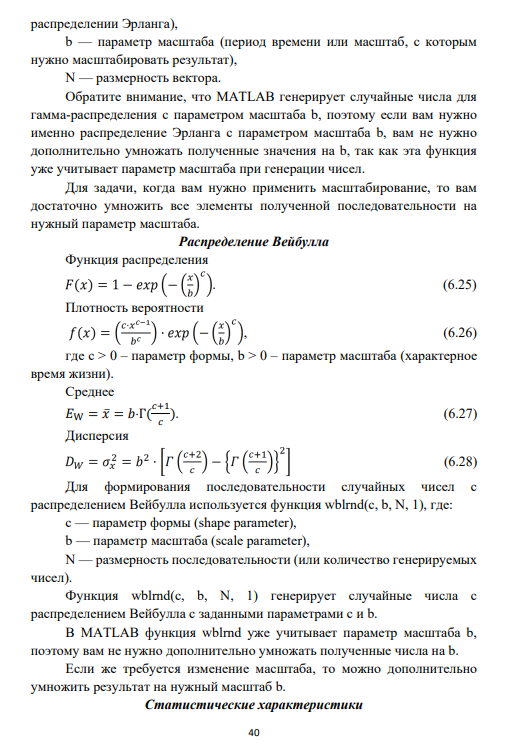
\includegraphics[width=1.0\textwidth]{theory6.png}
    \caption{Теория для лабораторной работы}
\end{figure}

\begin{figure}[H]
    \centering
    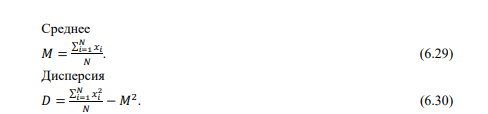
\includegraphics[width=1.0\textwidth]{theory7.png}
    \caption{Теория для лабораторной работы}
\end{figure}



\endinput